\documentclass[11pt,compress,t,notes=noshow, xcolor=table]{beamer}
\usepackage[]{graphicx}\usepackage[]{color}
% maxwidth is the original width if it is less than linewidth
% otherwise use linewidth (to make sure the graphics do not exceed the margin)
\makeatletter
\def\maxwidth{ %
  \ifdim\Gin@nat@width>\linewidth
    \linewidth
  \else
    \Gin@nat@width
  \fi 
}
\makeatother

\definecolor{fgcolor}{rgb}{0.345, 0.345, 0.345}
\newcommand{\hlnum}[1]{\textcolor[rgb]{0.686,0.059,0.569}{#1}}%
\newcommand{\hlstr}[1]{\textcolor[rgb]{0.192,0.494,0.8}{#1}}%
\newcommand{\hlcom}[1]{\textcolor[rgb]{0.678,0.584,0.686}{\textit{#1}}}%
\newcommand{\hlopt}[1]{\textcolor[rgb]{0,0,0}{#1}}%
\newcommand{\hlstd}[1]{\textcolor[rgb]{0.345,0.345,0.345}{#1}}%
\newcommand{\hlkwa}[1]{\textcolor[rgb]{0.161,0.373,0.58}{\textbf{#1}}}%
\newcommand{\hlkwb}[1]{\textcolor[rgb]{0.69,0.353,0.396}{#1}}%
\newcommand{\hlkwc}[1]{\textcolor[rgb]{0.333,0.667,0.333}{#1}}%
\newcommand{\hlkwd}[1]{\textcolor[rgb]{0.737,0.353,0.396}{\textbf{#1}}}%
\let\hlipl\hlkwb

\usepackage{framed}
\makeatletter
\newenvironment{kframe}{%
 \def\at@end@of@kframe{}%
 \ifinner\ifhmode%
  \def\at@end@of@kframe{\end{minipage}}%
  \begin{minipage}{\columnwidth}%
 \fi\fi%
 \def\FrameCommand##1{\hskip\@totalleftmargin \hskip-\fboxsep
 \colorbox{shadecolor}{##1}\hskip-\fboxsep
     % There is no \\@totalrightmargin, so:
     \hskip-\linewidth \hskip-\@totalleftmargin \hskip\columnwidth}%
 \MakeFramed {\advance\hsize-\width
   \@totalleftmargin\z@ \linewidth\hsize
   \@setminipage}}%
 {\par\unskip\endMakeFramed%
 \at@end@of@kframe}
\makeatother

\definecolor{shadecolor}{rgb}{.97, .97, .97}
\definecolor{messagecolor}{rgb}{0, 0, 0}
\definecolor{warningcolor}{rgb}{1, 0, 1}
\definecolor{errorcolor}{rgb}{1, 0, 0}
\newenvironment{knitrout}{}{} % an empty environment to be redefined in TeX

\usepackage{alltt}
\newcommand{\SweaveOpts}[1]{}  % do not interfere with LaTeX
\newcommand{\SweaveInput}[1]{} % because they are not real TeX commands
\newcommand{\Sexpr}[1]{}       % will only be parsed by R



\usepackage[english]{babel}
\usepackage[utf8]{inputenc}

\usepackage{dsfont}
\usepackage{verbatim}
\usepackage{amsmath}
\usepackage{amsfonts}
\usepackage{bm}
\usepackage{csquotes}
\usepackage{multirow}
\usepackage{longtable}
\usepackage{booktabs}
\usepackage{enumerate}
\usepackage[absolute,overlay]{textpos}
\usepackage{psfrag}
\usepackage{algorithm}
\usepackage{algpseudocode}
\usepackage{eqnarray}
\usepackage{arydshln}
\usepackage{tabularx}
\usepackage{placeins}
\usepackage{tikz}
\usepackage{setspace}
\usepackage{colortbl}
\usepackage{mathtools}
\usepackage{wrapfig}
\usepackage{bm}
\usepackage{xcolor}
\usetikzlibrary{shapes,arrows,automata,positioning,calc,chains,trees, shadows}
\tikzset{
  %Define standard arrow tip
  >=stealth',
  %Define style for boxes
  punkt/.style={
    rectangle,
    rounded corners,
    draw=black, very thick,
    text width=6.5em,
    minimum height=2em,
    text centered},
  % Define arrow style
  pil/.style={
    ->,
    thick,
    shorten <=2pt,
    shorten >=2pt,}
}
\usepackage{subfig}


% Defines macros and environments
\input{../../style/common.tex}

%\usetheme{lmu-lecture}
% \newcommand{\titlefigure}{figure/ml-basic-riskmin-error-surface.png}
% \newcommand{\learninggoals}{\item Know the concept of loss \item Understand the relationship between loss and risk \item Understand the relationship between risk minimization and finding the best model}
\usepackage{fancy}

\colorlet{GRAY}{gray}

\let\code=\texttt
\let\proglang=\textsf

\setkeys{Gin}{width=0.9\textwidth}

\title{Models in Machine Learning}
% \author{Bernd Bischl, Christoph Molnar, Daniel Schalk, Fabian Scheipl}
\institute{\href{https://compstat-lmu.github.io/lecture_i2ml/}{compstat-lmu.github.io/lecture\_i2ml}}
\date{}

\setbeamertemplate{frametitle}{\expandafter\uppercase\expandafter\insertframetitle}



\begin{document}
% Introduction to Machine Learning
% Day 1

% Set style/preamble.Rnw as parent.

% Load all R packages and set up knitr

% This file loads R packages, configures knitr options and sets preamble.Rnw as parent file
% IF YOU MODIFY THIS, PLZ ALSO MODIFY setup.Rmd ACCORDINGLY...

% Defines macros and environments
\input{../../latex-math/basic-math.tex}
\input{../../latex-math/basic-ml.tex}
\input{../../latex-math/ml-lm.tex}
\input{../../latex-math/ml-trees.tex}
% \input{../../latex-math/ml-rf.tex}
\input{../../latex-math/ml-bagging.tex}
\input{../../latex-math/ml-boosting.tex}

%! includes: basics-learners

\lecturechapter{An Overview}
\lecture{Models in Machine Learning}

\begin{frame}{Disclaimer}

\textcolor{red}{In machine learning, there’s something called the “No Free 
Lunch” theorem. In a nutshell, it states that no one algorithm works best for 
every problem, and it’s 
especially relevant for supervised learning (i.e. predictive modeling).
For example, you can’t say that neural networks are always better than decision 
trees or vice-versa. There are many factors at play, such as the size and 
structure of your dataset.
As a result, you should try many different algorithms for your problem, while 
using a hold-out “test set” of data to evaluate performance and select the 
winner.}

\end{frame}

% ------------------------------------------------------------------------------
% CART (Classification and Regression Trees)
% ------------------------------------------------------------------------------

% \LARGE
% \begin{frame}{\textcolor{gray!80}{CART} ~~ Functionality}
% \normalsize
% \vspace{-0.5cm}
% \noindent \textcolor{gray!80}{\rule{\textwidth}{1pt}}
% 
% \vspace{0.2cm}
% 
% \scriptsize
% 
% \colorbox{gray!80}{\textcolor{white}{SUPERVISED}} 
% \colorbox{gray!80}{\textcolor{white}{NON-PARAMETRIC}} 
% \colorbox{gray!80}{\textcolor{white}{WHITE-BOX}} 
% \colorbox{gray!80}{\textcolor{white}{FEATURE SELECTION}}
% 
% \medskip
% 
% \textbf{\textcolor{gray!80}{General idea}} {}{} Starting from a root node, 
% \textit{\textbf{classification \& regression trees (CART)}} 
% perform repeated \textbf{binary splits} of the data according to feature values, 
% thereby subsequently dividing the input space $\Xspace$ into $M$ 
% \textbf{rectangular partitions}.
% 
% \begin{itemize}
%   \item [$\rightarrow$] Pass observations along until each ends up in exactly 
%   one leaf node
%   \item [$\rightarrow$] In each step, find the optimal feature-threshold
%   combination to split by
%   \item [$\rightarrow$] Assign response $c_m$ to leaf node $m$
% \end{itemize}
% 
% \vspace{0.1cm}
% 
% \begin{minipage}{0.6\textwidth}
%   \textbf{\textcolor{gray!80}{Hypothesis space}} \\
%   $$\Hspace = \left\{ \fx: \fx = \sum_{m = 1}^M c_m \mathbb{I}(\xv \in Q_m) 
%   \right\}$$
%   \medskip
%   \textbf{\textcolor{gray!80}{Loss functions}} \\
%   Classification: mostly \textit{\textbf{Brier score, Bernoulli loss}}  \\
%   \medskip
%   Regression: mostly \textit{\textbf{quadratic loss}}
% \end{minipage}%
% \begin{minipage}{0.4\textwidth}
%   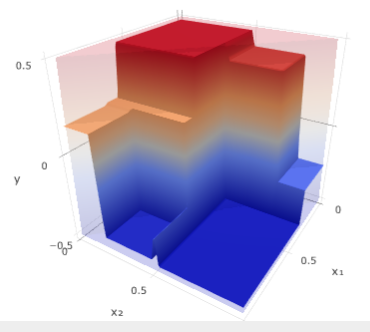
\includegraphics[width=0.8\textwidth]{figure/cart_3d.PNG}
% \end{minipage}
% 
% \medskip
% \textbf{\textcolor{gray!80}{Optimization}} {}{} Exhaustive search for optimal 
% splitting criterion (greedy optimization) \\
% \medskip
% \textbf{\textcolor{gray!80}{Hyperparameters}} {}{} Tree depth, minimum number
% of observations per node, ...
% 
% \end{frame}

% ------------------------------------------------------------------------------

\LARGE
\begin{frame}{\textcolor{gray!80}{CART} ~~ Functionality}
\normalsize
\vspace{-0.5cm}
\noindent \textcolor{gray!80}{\rule{\textwidth}{1pt}}

\vspace{0.3cm}

\footnotesize

\colorbox{gray!80}{\textcolor{white}{SUPERVISED}} 
\colorbox{gray!80}{\textcolor{white}{NON-PARAMETRIC}} 
\colorbox{gray!80}{\textcolor{white}{WHITE-BOX}} 
\colorbox{gray!80}{\textcolor{white}{FEATURE SELECTION}}

\medskip

\textbf{\textcolor{gray!80}{General idea}} ~~ Starting from a root node, 
\textit{\textbf{classification \& regression trees (CART)}} 
perform repeated \textbf{binary splits} of the data according to feature values, 
thereby subsequently dividing the input space $\Xspace$ into $T$ 
\textbf{rectangular partitions} $Q_t$.

\medskip
 
\textbf{\textcolor{gray!80}{Hypothesis space}} ~~
$\Hspace = \left\{ \fx: \fx = \sum_{t = 1}^T c_t \I(\xv \in Q_t) 
\right\}$

\medskip

\begin{minipage}{0.6\textwidth}
  \begin{itemize}
    \item Pass observations along until each ends up in exactly 
    one leaf node
    \item In each step, find the optimal feature-threshold
    combination to \\ split by
  \item Assign response $c_t$ to leaf node $t$
\end{itemize}

\end{minipage}%
\begin{minipage}{0.4\textwidth}
  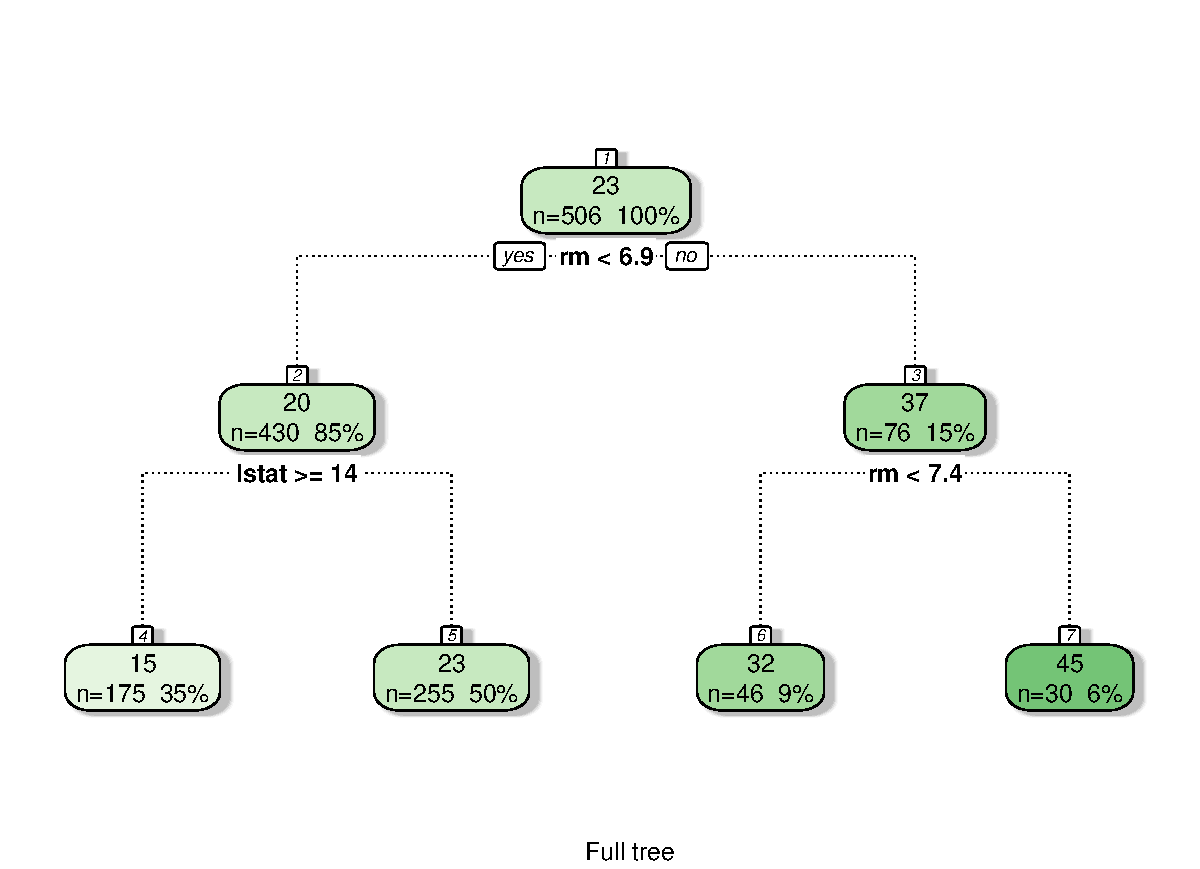
\includegraphics[width=\textwidth]{figure/cart.pdf}
\end{minipage}

\end{frame}

% ------------------------------------------------------------------------------

\LARGE
\begin{frame}{\textcolor{gray!80}{CART} ~~ Functionality}
\normalsize
\vspace{-0.5cm}
\noindent \textcolor{gray!80}{\rule{\textwidth}{1pt}}

\vspace{0.3cm}

\footnotesize

\textbf{\textcolor{gray!80}{Empirical risk}} \\

\begin{itemize}
  \item Empirical risk is calculated for each potential terminal node $\Np_t$
  of a split.
  \item In general, trees can handle any type of loss function. Typical choices
  are:
  \begin{itemize}
    \footnotesize
    \item Classification (for $g$ classes):
    \begin{itemize}
      \footnotesize
      \item Using \textit{\textbf{Brier score}} ~~
      $\risk(\Np_t) = \sum\limits_{(\xv,y) \in \Np_t} \sumkg \left( \I(y = k)
      - \pikx \right)^2$
      \item Using \textit{\textbf{Bernoulli loss}} ~~
      $\risk(\Np_t) = \sum\limits_{(\xv,y) \in \Np_t} \sumkg \I(y = k) \cdot
      \log(\pikx)$
    \end{itemize}
    \item Regression: Using \textit{\textbf{quadratic loss}} ~~
    $\risk(\Np_t) = \sum\limits_{(\xv,y) \in \Np_t} (y - c_t)^2$
  \end{itemize}
\end{itemize}

\medskip

\textbf{\textcolor{gray!80}{Optimization}} ~~ \textbf{Exhaustive} search over
all (randomly selected) split candidates in each node to minimize empirical risk 
in the child nodes (greedy optimization) \\

\medskip

\textbf{\textcolor{gray!80}{Hyperparameters}} ~~ \textbf{Complexity}, i.e., 
number of leaves $T$ \\

\normalsize
  
\end{frame}

% ------------------------------------------------------------------------------

\LARGE
\begin{frame}{\textcolor{gray!80}{CART} ~~ Pro's \& Con's}
\normalsize
\vspace{-0.5cm}
\noindent \textcolor{gray!80}{\rule{\textwidth}{1pt}}

\vspace{0.3cm}

\footnotesize

\begin{columns}[onlytextwidth]
  \begin{column}{0.5\textwidth}
    \textbf{\textcolor{gray!80}{Advantages}}
    \footnotesize
    \begin{itemize}
      \item[$\textbf{\textcolor{gray!80}{+}}$] \textbf{Easy} to understand, 
      interpret \& visualize
      \item[$\textbf{\textcolor{gray!80}{+}}$] Automatic handling of 
      \textbf{non-numerical} features
      \item[$\textbf{\textcolor{gray!80}{+}}$] Built-in \textbf{feature 
      selection}
      \item[$\textbf{\textcolor{gray!80}{+}}$] Automatic handling of 
      \textbf{missings} 
      \item[$\textbf{\textcolor{gray!80}{+}}$] \textbf{Interaction} effects 
      between features easily possible, even of higher orders
      \item[$\textbf{\textcolor{gray!80}{+}}$] \textbf{Fast} computation and 
      good scalability
      \item[$\textbf{\textcolor{gray!80}{+}}$] High \textbf{flexibility} (custom 
      split criteria or leaf-node prediction rules)   
    \end{itemize}
  \end{column}
  \begin{column}{0.5\textwidth}
    \textbf{\textcolor{gray!80}{Disadvantages}}
    \footnotesize
    \begin{itemize}
      \item[$\textbf{\textcolor{gray!80}{-}}$] Rather \textbf{low accuracy} (at 
      least, without bagging or boosting)
      \item[$\textbf{\textcolor{gray!80}{-}}$] High 
      \textbf{variance/instability}: strong dependence on training data
      \item[$\textbf{\textcolor{gray!80}{-}}$] Therefore, poor generalization \& 
      risk of \textbf{overfitting}
      \item[$\textbf{\textcolor{gray!80}{-}}$] Several steps required for
      modeling \textbf{linear} relationships
      \item[$\textbf{\textcolor{gray!80}{-}}$] In presence of categorical 
      features, \textbf{bias} towards features with \textbf{many categories}
    \end{itemize}
  \end{column}
\end{columns}

\vfill

\small

\fbox{\parbox{\textwidth}{
\centering
\textbf{Simple and good with feature selection, but not the best
predictor}}}

\end{frame}

% ------------------------------------------------------------------------------

\LARGE
\begin{frame}{\textcolor{gray!80}{CART} ~~ Practical hints}
\normalsize
\vspace{-0.5cm}
\noindent \textcolor{gray!80}{\rule{\textwidth}{1pt}}

\vspace{0.3cm}

\footnotesize

\textbf{\textcolor{gray!80}{Pruning / early stopping}} \\
\smallskip
Unless interrupted, splitting will go on until each leaf node contains a single 
observation (expensive + overfitting!) \\
\smallskip
$\rightarrow$ Use \textbf{pruning} and \textbf{stopping criteria} to limit 
complexity

\lz
\textbf{\textcolor{gray!80}{Implementation}} \\
\smallskip
R: package \texttt{rpart}\\
Python: \texttt{DecisionTreeClassifier} / \texttt{DecisionTreeRegressor} from 
package \texttt{scikit-learn} \\
Complexity controlled via tree depth, minimum number of observations per 
node, maximum number of leaves, minimum risk reduction per split, ...

\lz
\textbf{\textcolor{gray!80}{Bagging / boosting}} \\
\smallskip
Since CART are instable predictors on their own, they are typically ensembled
to form a \textit{\textbf{random forest}} (\textit{\textbf{bagging}}) or used in 
combination with \textit{\textbf{boosting}}.

\end{frame}

% ------------------------------------------------------------------------------
% RANDOM FORESTS
% ------------------------------------------------------------------------------

\LARGE
\begin{frame}{\textcolor{gray!80}{Random forests} ~~ Functionality}
\normalsize
\vspace{-0.5cm}
\noindent \textcolor{gray!80}{\rule{\textwidth}{1pt}}

\vspace{0.3cm}

\footnotesize

\colorbox{gray!80}{\textcolor{white}{SUPERVISED}} 
\colorbox{gray!80}{\textcolor{white}{NON-PARAMETRIC}} 
\colorbox{gray!80}{\textcolor{white}{BLACK-BOX}} 
\colorbox{gray!80}{\textcolor{white}{FEATURE SELECTION}}

\medskip

\textbf{\textcolor{gray!80}{General idea}} ~~ Random forests are 
\textit{\textbf{bagging ensembles}}: they combine multiple CART (base learners)
to form a strong learner. They use \textbf{complex} trees with low  bias and 
compensate for single trees' high variance by aggregating $M$ of them in a 
\textbf{decorrelated} manner. 

\medskip

\textbf{\textcolor{gray!80}{Hypothesis space}} ~~
$\Hspace = \left\{ \fx: \fx = \frac{1}{M} \sum_{m = 1}^M \sum_{t = 1}^{T^{[m]}} 
c_t^{[m]} \I(\xv \in Q_t^{[m]}) \right\}$

\medskip

\begin{minipage}{0.6\textwidth}
  \begin{itemize}
    \item Training on bootstrap samples of the data and only on a random subset 
    of features to incur variability
    \item Aggregation via averaging (regression) or majority voting
    (classification)
  \end{itemize}
\end{minipage}%
\begin{minipage}{0.4\textwidth}
  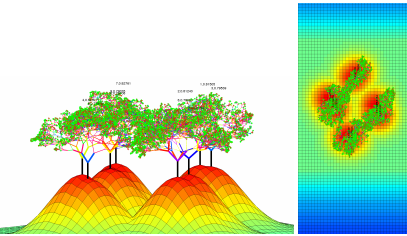
\includegraphics[width=0.9\textwidth]{figure/rf_3d.PNG}
\end{minipage}

\end{frame}

% ------------------------------------------------------------------------------

\LARGE
\begin{frame}{\textcolor{gray!80}{Random forests} ~~ Functionality}
\normalsize
\vspace{-0.5cm}
\noindent \textcolor{gray!80}{\rule{\textwidth}{1pt}}

\vspace{0.3cm}

\footnotesize

\textbf{\textcolor{gray!80}{Empirical risk}} ~~
Applicable with \textbf{any} kind of loss function (just like tree base 
learners) \\
$\rightarrow$ Computation of empirical risk for all potential child nodes in all 
trees

\medskip

\textbf{\textcolor{gray!80}{Optimization}} ~~ \textbf{Exhaustive} search over
all (randomly selected) split candidates in each node of each tree to minimize
empirical risk in the child nodes (greedy optimization) \\

\medskip

\textbf{\textcolor{gray!80}{Hyperparameters}}

\begin{itemize}
  \item \textbf{Ensemble size}, i.e., number of trees
  \item \textbf{Complexity}, i.e., number of leaves $T$ of each base learner
  \item \textbf{Number of split candidates}, i.e., number of features to be
  considered as splitting variables at each split \\
  $\rightarrow$ Frequently used heuristics: 
  $\left \lfloor{\sqrt{p}}\right \rfloor$ for classification and
  $\left \lfloor{p/3}\right \rfloor$ for regression
\end{itemize}
  
\end{frame}


% ------------------------------------------------------------------------------

\LARGE
\begin{frame}{\textcolor{gray!80}{Random forests} ~~ Pro's \& Con's}
\normalsize
\vspace{-0.5cm}
\noindent \textcolor{gray!80}{\rule{\textwidth}{1pt}}

\vspace{0.3cm}

\footnotesize

\begin{columns}[onlytextwidth]
  \begin{column}{0.5\textwidth}
    \textbf{\textcolor{gray!80}{Advantages}}
    \footnotesize
    \begin{itemize}
      \item[$\textbf{\textcolor{gray!80}{+}}$] Translation of most of 
      \textbf{base learners'} advantages (e.g., inherent variable selection, 
      handling of missing data)
      \item[$\textbf{\textcolor{gray!80}{+}}$] Fairly good at 
      \textbf{prediction}: improved accuracy through bagging
      \item[$\textbf{\textcolor{gray!80}{+}}$] Inherent computation of 
      \textbf{feature importance}
      \item[$\textbf{\textcolor{gray!80}{+}}$] Quite \textbf{stable} wrt changes 
      in the data
      \item[$\textbf{\textcolor{gray!80}{+}}$] Good with 
      \textbf{high-dimensional} data, even in presence of noisy covariates
      \item[$\textbf{\textcolor{gray!80}{+}}$] Applicable to \textbf{unbalanced} 
      data
      \item[$\textbf{\textcolor{gray!80}{+}}$] Easy to \textbf{parallelize}
      \item[$\textbf{\textcolor{gray!80}{+}}$] Rather easy to \textbf{tune}
    \end{itemize}
  \end{column}
  \begin{column}{0.5\textwidth}
    \textbf{\textcolor{gray!80}{Disadvantages}}
    \footnotesize
    \begin{itemize}
      \item[$\textbf{\textcolor{gray!80}{-}}$] Translation of some of 
      \textbf{base learners'} disadvantages (e.g., trouble to model linear
      relations, bias towards features with many categories)
      \item[$\textbf{\textcolor{gray!80}{-}}$] Loss of single trees' 
      \textbf{interpretability} -- black-box method
      \item[$\textbf{\textcolor{gray!80}{-}}$] Hard to \textbf{visualize}
      \item[$\textbf{\textcolor{gray!80}{-}}$] Often suboptimal for 
      \textbf{regression}
      \item[$\textbf{\textcolor{gray!80}{-}}$] Often still inferior in
      \textbf{performance} to other methods (e.g., boosting)
    \end{itemize}
  \end{column}
\end{columns}

\vfill

\small

\fbox{\parbox{\textwidth}{
\centering
\textbf{Fairly good predictor, but black-box method}}}

\end{frame}

% ------------------------------------------------------------------------------

\LARGE
\begin{frame}{\textcolor{gray!80}{Random forests} ~~ Practical hints}
\normalsize
\vspace{-0.5cm}
\noindent \textcolor{gray!80}{\rule{\textwidth}{1pt}}

\vspace{0.3cm}

\footnotesize

\textbf{\textcolor{gray!80}{Pre-processing}} \\
\smallskip
Inherent feature selection of random forests, but high \textbf{computational 
costs} for large number of features \\
$\rightarrow$ Upstream feature selection (e.g., via PCA) might be advisable
\lz

\textbf{\textcolor{gray!80}{Implementation}} \\
\smallskip
R: package \texttt{ranger}\\
Python: \texttt{RandomForestClassifier} / \texttt{RandomForestRegressor} from 
package \texttt{scikit-learn}
\lz

\textbf{\textcolor{gray!80}{Tuning}} \\
\smallskip
Overall \textbf{limited tunability} \\
Number of split candidates often more impactful than number of trees

\end{frame}

% ------------------------------------------------------------------------------
% GRADIENT BOOSTING
% ------------------------------------------------------------------------------

\LARGE
\begin{frame}{\textcolor{gray!80}{Gradient Boosting} ~~ Functionality}
\normalsize
\vspace{-0.5cm}
\noindent \textcolor{gray!80}{\rule{\textwidth}{1pt}}

\vspace{0.3cm}

\footnotesize

\colorbox{gray!80}{\textcolor{white}{SUPERVISED}} 
\colorbox{gray!80}{\textcolor{white}{NON-PARAMETRIC}} 
\colorbox{gray!80}{\textcolor{white}{BLACK-BOX}}
\colorbox{gray!80}{\textcolor{white}{FEATURE SELECTION}}

\medskip

\textbf{\textcolor{gray!80}{General idea}} ~~ Gradient boosting (GB) is an
\textit{\textbf{ensemble}} method that constructs a strong learner from weak 
base learners (frequently, CART). \\
As opposed to \textit{\textbf{bagging}}, however, base learners are assembled
in a \textbf{sequential, stage-wise} manner: in each iteration, GB improves the 
current model by adding a new component that minimizes empirical risk. The final 
model is a weighted sum of base learners $b(\xv, \thetam)$ with weights 
$\betam$.

\medskip

\textbf{\textcolor{gray!80}{Hypothesis space}} ~~
$\Hspace = \left\{ \fx: \fx = \sum_{m = 1}^M \betam b(\xv, \thetam) \right\}$

\medskip

\begin{minipage}{0.6\textwidth}
  \begin{itemize}
    \item Finding next additive component $\widehat{=}$ fitting base learner
    to current point-wise residuals  
    \item One boosting iteration $\widehat{=}$ one approximate gradient step in 
    function space
    \item Fitting of each base learner using information from previously
    added ones
  \end{itemize}
\end{minipage}%
\begin{minipage}{0.4\textwidth}
  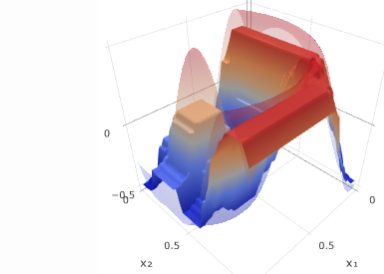
\includegraphics[width=0.9\textwidth]{figure/gb_3d.PNG}
\end{minipage}

\end{frame}

% ------------------------------------------------------------------------------

\LARGE
\begin{frame}{\textcolor{gray!80}{Gradient boosting} ~~ Functionality}
\normalsize
\vspace{-0.5cm}
\noindent \textcolor{gray!80}{\rule{\textwidth}{1pt}}

\vspace{0.3cm}

\footnotesize

\textbf{\textcolor{gray!80}{Empirical risk}}

\begin{itemize}
  \item \textbf{Outer loss:} Loss used to compute pseudo-residuals -- how large 
  is the error of the current model fit? \\
  $\rightarrow$ Arbitrary \textbf{differentiable} loss function
  \item \textbf{Inner loss:} Loss used to fit next base learner component to 
  current pseudo-residuals \\
  $\rightarrow$ Typically, \textit{\textbf{quadratic loss}} (desirable 
  optimization properties)
\end{itemize}

\medskip

\textbf{\textcolor{gray!80}{Optimization}} ~~ \textit{\textbf{Functional 
gradient descent}} for outer optimization loop, procedure for inner one 
depending on inner loss

\medskip

\textbf{\textcolor{gray!80}{Hyperparameters}}

\begin{itemize}
  \item \textbf{Ensemble size}, i.e., number of base learners
  \item \textbf{Learning rate}, i.e., impact of single base learner
  \item \textbf{Complexity} of base learners (depending on type used)
\end{itemize}

\end{frame}

% ------------------------------------------------------------------------------

\LARGE
\begin{frame}{\textcolor{gray!80}{Gradient Boosting} ~~ Pro's \& Con's}
\normalsize
\vspace{-0.5cm}
\noindent \textcolor{gray!80}{\rule{\textwidth}{1pt}}

\vspace{0.3cm}

\footnotesize

\begin{columns}[onlytextwidth]
  \begin{column}{0.5\textwidth}
    \textbf{\textcolor{gray!80}{Advantages}}
    \footnotesize
    \begin{itemize}
      \item[$\textbf{\textcolor{gray!80}{+}}$] Powerful \textbf{off-the-shelf}
      method for supercharging weak learners' performance
      \item[$\textbf{\textcolor{gray!80}{+}}$] Translation of most of 
      \textbf{base learners'} advantages (e.g., for tree boosting: inherent 
      variable selection, handling of missing data)
      \item[$\textbf{\textcolor{gray!80}{+}}$] High predictive
      \textbf{accuracy} that is hard to outperform
      \item[$\textbf{\textcolor{gray!80}{+}}$] High \textbf{flexibility} (custom
      loss functions, many tuning options) 
      \item[$\textbf{\textcolor{gray!80}{+}}$] Applicable to \textbf{unbalanced} 
      data
    \end{itemize}
  \end{column}
  \begin{column}{0.5\textwidth}
    \textbf{\textcolor{gray!80}{Disadvantages}}
    \footnotesize
    \begin{itemize}
      \item[$\textbf{\textcolor{gray!80}{-}}$] Hardly
      \textbf{interpretable} -- black-box method
      \item[$\textbf{\textcolor{gray!80}{-}}$] Hard to \textbf{visualize}
      \item[$\textbf{\textcolor{gray!80}{-}}$] Prone to \textbf{overfitting}
      \item[$\textbf{\textcolor{gray!80}{-}}$] Sensitive to \textbf{outliers}
      \item[$\textbf{\textcolor{gray!80}{-}}$] Hard to \textbf{tune} (high
      sensitivity to variations in hyperparameter values)
      \item[$\textbf{\textcolor{gray!80}{-}}$] Rather \textbf{slow} in training
      \item[$\textbf{\textcolor{gray!80}{-}}$] Hard to \textbf{parallelize}
    \end{itemize}
  \end{column}
\end{columns}

\vfill

\small

\fbox{\parbox{\textwidth}{
\centering
\textbf{High-performing predictor, but rather delicate to handle}}}

\end{frame}

% ------------------------------------------------------------------------------

\LARGE
\begin{frame}{\textcolor{gray!80}{Gradient Boosting} ~~ Practical hints}
\normalsize
\vspace{-0.5cm}
\noindent \textcolor{gray!80}{\rule{\textwidth}{1pt}}

\vspace{0.3cm}

\footnotesize

\textbf{\textcolor{gray!80}{XGBoost (extreme gradient boosting)}} \\
\smallskip
Fast, efficient implementation of gradient-boosted decision trees that has
become \textbf{state of the art} for many machine learning problems \\
$\rightarrow$ Clever modeling techniques + computational speed \\

\lz

\textbf{\textcolor{gray!80}{Stochastic gradient boosting (SGB)}} \\
\smallskip
Faster, approximate version of GB that performs each iteration only on 
\textbf{random subset} of the data \\
$\rightarrow$ Potentially preferrable for high-dimensional data sets 

\lz

\textbf{\textcolor{gray!80}{Implementation}} \\
\smallskip
R: packages \texttt{gbm}, \texttt{xgboost}\\
Python: \texttt{GradientBoostingClassifier} / \texttt{GradientBoostingRegressor} 
from package \texttt{scikit-learn}, \texttt{XGBClassifier} / 
\texttt{XGBRegressor} from package \texttt{xgboost}
\lz

\textbf{\textcolor{gray!80}{Tuning}} \\
\smallskip
Overall \textbf{limited tunability} \\
Number of split candidates often more impactful than number of trees

\end{frame}

% ------------------------------------------------------------------------------




%----------------------------------------------------------------------------------------
%=========================================================================================
%-----------------------------------------------------------------------------------------




% ------------------------------------------------------------------------------
% LINEAR MODEL
% ------------------------------------------------------------------------------

\LARGE
\begin{frame}{\textcolor{gray!80}{Linear Model} ~~ Functionality}
\normalsize
\vspace{-0.5cm}
\noindent \textcolor{gray!80}{\rule{\textwidth}{1pt}}

\vspace{0.3cm}

\footnotesize

\colorbox{gray!80}{\textcolor{white}{SUPERVISED}} 
\colorbox{gray!80}{\textcolor{white}{PARAMETRIC}} 
\colorbox{gray!80}{\textcolor{white}{WHITE-BOX}}
%\colorbox{gray!80}{\textcolor{white}{FEATURE SELECTION}}

\medskip

\textbf{\textcolor{gray!80}{General idea}} ~~  
%\begin{itemize}
A linear model (LM) fits a \textbf{hyperplane} $\theta_0 + \thx$ to minimize the distance between the data points and its closed point on the hyperplane. 
%\item The linear model approximates the \textbf{linear influence} of the features on the target variable. 
%\item Thus, linear models can only perform \textbf{regression}, as they can only predict continous, numeric values. 
%\end{itemize}

\medskip

\textbf{\textcolor{gray!80}{Hypothesis space}} ~~
$\Hspace = \{ \theta_0 + \thx\ |\ (\theta_0, \thetab) \in \R^{p+1} \}$

% \textbf{Linear Model}: Used in different contexts, often a synonym for models in the class of linear predictors or for linear regression (with potentially transformed input space, i.e.,  $\yi = \thetab^\top \psi^{(i)}(\xi) + \varepsilon^{(i)}$, where $\psi^{(i)}(\cdot)$ can be non-linear functions transforming $\xi$). 


\medskip
\footnotesize
\begin{minipage}{0.45\textwidth}
  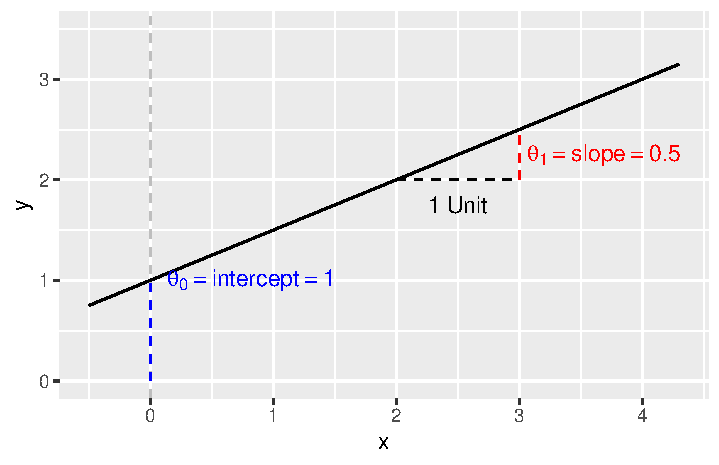
\includegraphics[width=0.8\textwidth]{figure/reg_lm_plot.pdf}
\end{minipage}
 \normalsize 
\begin{minipage}{0.45\textwidth}
  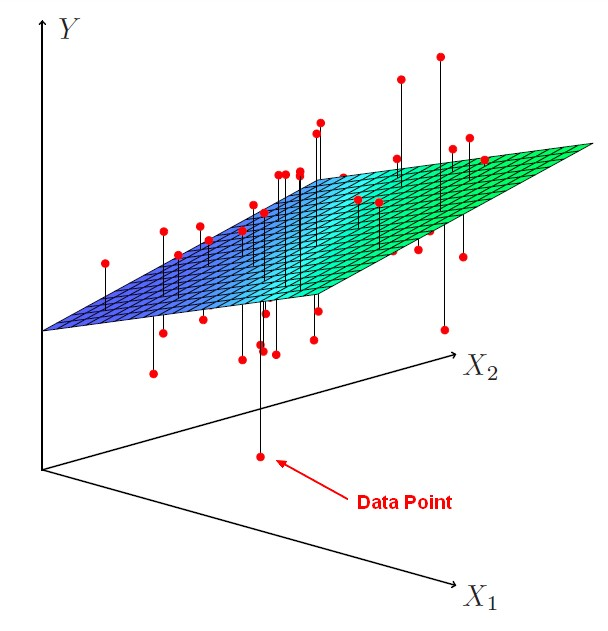
\includegraphics[width=0.7\textwidth]{figure/regression_hyperplane.jpg}
\end{minipage}

\end{frame}

% ------------------------------------------------------------------------------

\LARGE
\begin{frame}{\textcolor{gray!80}{Linear model} ~~ Functionality}
\normalsize
\vspace{-0.5cm}
\noindent \textcolor{gray!80}{\rule{\textwidth}{1pt}}

\vspace{0.3cm}




\footnotesize

\textbf{\textcolor{gray!80}{Empirical risk}}
\begin{itemize}\footnotesize
  \item Typically, \textbf{ordinary least squares (OLS)} with a squared loss function is used for regression: $\risket  = \sumin \left(\yi - \thetab^T \xi\right)^2$
    
   \item Sometimes the empirical risk function is based on the \textbf{absolute loss} or the \textbf{Huber loss}. %$\risket = \sumin \left|\yi - \thetab^T \xi\right|$ 
  
  \item For \textbf{logistic regression} the ERM is based on the \textbf{log loss} $\Lxy = \log \left[1 + \exp \left(-y\fx\right)\right]$.
  
  \item In this case, the hyperplane can represent the decision boundary between two classes (\textbf{classification}). 


\end{itemize}

\footnotesize

\medskip

\textbf{\textcolor{gray!80}{Optimization}} ~~ 
\begin{itemize}\footnotesize
  \item for \textbf{OLS}: analytically with $\bm{\hat \theta} = (\Xmat^\top \Xmat)^{-1} \Xmat^\top\ydat$
  \item for \textbf{other loss functions}: numerical optimization 
\end{itemize}

\medskip

\textbf{\textcolor{gray!80}{Hyperparameters}} ~~ none

\end{frame}

% ------------------------------------------------------------------------------

\LARGE
\begin{frame}{\textcolor{gray!80}{Linear model} ~~ Pro's \& Con's}
\normalsize
\vspace{-0.5cm}
\noindent \textcolor{gray!80}{\rule{\textwidth}{1pt}}

\vspace{0.3cm}

\footnotesize

\begin{columns}[onlytextwidth]
  \begin{column}{0.5\textwidth}
    \textbf{\textcolor{gray!80}{Advantages}}
    \footnotesize
    \begin{itemize}
      \item[$\textbf{\textcolor{gray!80}{+}}$] \textbf{simple and fast} implementation; cheap computational costs
      \item[$\textbf{\textcolor{gray!80}{+}}$] intuitive \textbf{interpretability}: mean influence of features on the output and feature importance
      \item[$\textbf{\textcolor{gray!80}{+}}$] fits \textbf{linearly} separable data sets very well
      \item[$\textbf{\textcolor{gray!80}{+}}$] works well \textbf{independent of data size}
      \item[$\textbf{\textcolor{gray!80}{+}}$] basis for many machine learning algorithms

    \end{itemize}
  \end{column}

  \begin{column}{0.5\textwidth}
    \textbf{\textcolor{gray!80}{Disadvantages}}
    \footnotesize
    \begin{itemize}
      \item[$\textbf{\textcolor{gray!80}{-}}$] not suitable for data based on a \textbf{non-linear} data generating process $\rightarrow$ \textbf{strong simplification} of real-world problems
      
      \item[$\textbf{\textcolor{gray!80}{-}}$] \textbf{strong assumptions}: data is independent (multi-collinearity must be removed and normal distributed residuals ??
      
      \item[$\textbf{\textcolor{gray!80}{-}}$] tend to \textbf{overfit} (can be reduced by regularization)
      
      \item[$\textbf{\textcolor{gray!80}{-}}$] \textbf{sensitive to outliers and noisy data}
    \end{itemize}
  \end{column}
\end{columns}

\vfill

\small

\fbox{\parbox{\textwidth}{
\centering
\textbf{Simple method with good interpretability for linear problems, but strong assumptions and simplification of real-world problems}}}

\end{frame}

% ------------------------------------------------------------------------------

\LARGE
\begin{frame}{\textcolor{gray!80}{Linear Model} ~~ Practical hints}
\normalsize
\vspace{-0.5cm}
\noindent \textcolor{gray!80}{\rule{\textwidth}{1pt}}

\vspace{0.3cm}

\footnotesize

 \textbf{\textcolor{gray!80}{Check assumptions???????}} \\
 This model is very effective, if the following assumptions are fulfilled:
 \begin{itemize}\footnotesize
  \item \textbf{linearity}: the relationship between the mean of predicted value and the features
  \item \textbf{homoscedasticity}: The variance of residuals is equal for all features.
  \item \textbf{independence}: All observations are independent of each other.
  \item \textbf{normality}: Y is normally distributed for any fixed value of the features
\end{itemize}

\lz

  \textbf{\textcolor{gray!80}{Implementation}} \\
  \smallskip
  R: function \texttt{lm}\\
  Python: \texttt{LinearRegression} from package \texttt{sklearn.linear\_model}, package for advanced statistical parameters \texttt{statsmodels.api} 

\lz

 \textbf{\textcolor{gray!80}{Regularization}} \\
 \smallskip
 
 In practice, we often use regularized models in order to \textbf{prevent overfitting} or perform feature selection. More details will follow in the subsequent chapter. 


\end{frame}

% ------------------------------------------------------------------------------



% 
% 
% % ------------------------------------------------------------------------------
% % REGULARIZED LINEAR MODEL
% % ------------------------------------------------------------------------------

\LARGE
\begin{frame}{\textcolor{gray!80}{Regularized LM} ~~ Functionality}
\normalsize
\vspace{-0.5cm}
\noindent \textcolor{gray!80}{\rule{\textwidth}{1pt}}

\vspace{0.3cm}

\footnotesize

\colorbox{gray!80}{\textcolor{white}{SUPERVISED}}
\colorbox{gray!80}{\textcolor{white}{PARAMETRIC}}
\colorbox{gray!80}{\textcolor{white}{WHITE-BOX}}
%\colorbox{gray!80}{\textcolor{white}{REGRESSION}}
%\colorbox{gray!80}{\textcolor{white}{FEATURE SELECTION}}

\medskip

\textbf{\textcolor{gray!80}{General idea}} ~~
\begin{itemize}

\item Linear model (LM) can \textbf{overfit} if we operate in high-dimensional space with not that many oberservations.

\item When features are highly correlated, the least-squares estimate becomes highly sensitive to random errors in the observed response, producing a \textbf{large variance in the fit}.

\item If we fit a linear model, we can find a compromise between generalizing the model (simple model, underfitted) and correspond closely to the data (complex model, overfitted).

\end{itemize}

\medskip

\textbf{\textcolor{gray!80}{Hypothesis space}} ~~
$\Hspace = \{ \theta_0 + \thx\ |\ (\theta_0, \thetab) \in \R^{p+1} \} $

\medskip
% \footnotesize
% \begin{minipage}{0.5\textwidth}
\centering
  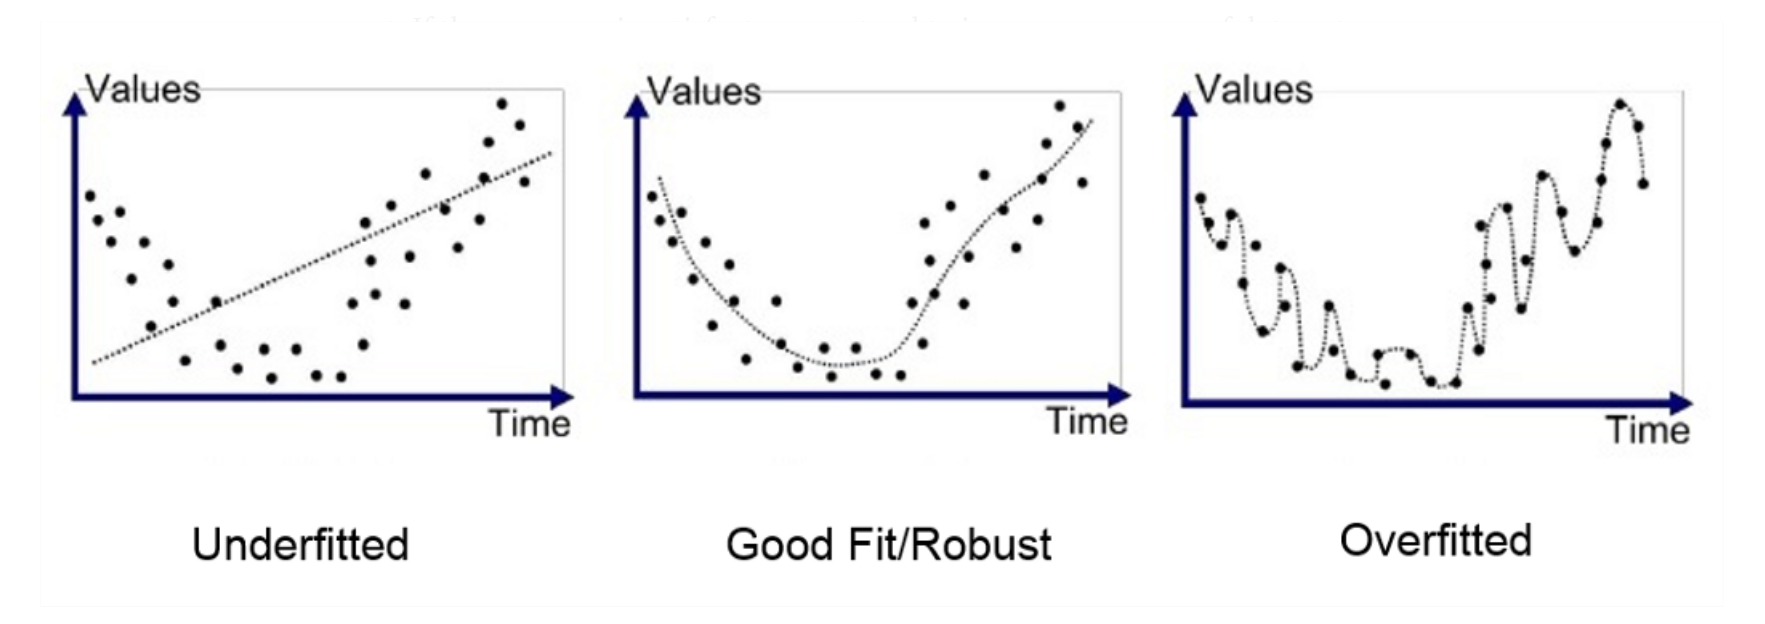
\includegraphics[width=0.7\textwidth]{figure/reg_lm_comparision.png}
% \end{minipage}
%  \normalsize
% \begin{minipage}{0.4\textwidth}
%   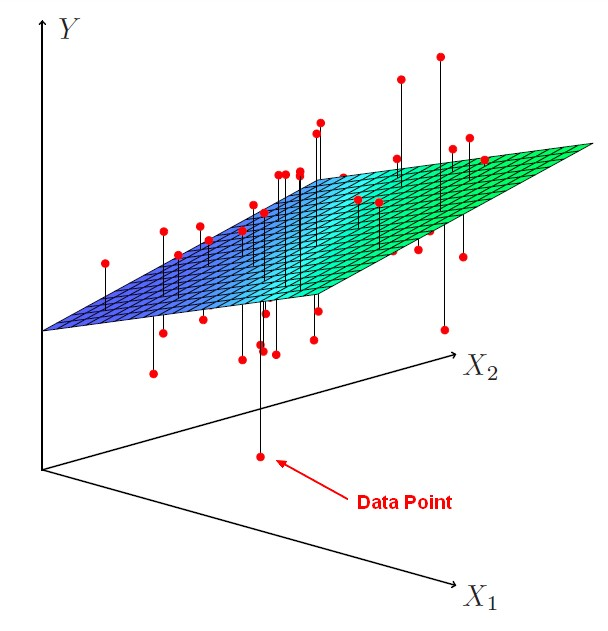
\includegraphics[width=0.7\textwidth]{figure/regression_hyperplane.jpg}
% \end{minipage}

\end{frame}

% ------------------------------------------------------------------------------

\LARGE
\begin{frame}{\textcolor{gray!80}{Regularized LM} ~~ Functionality}
\normalsize
\vspace{-0.5cm}
\noindent \textcolor{gray!80}{\rule{\textwidth}{1pt}}

\vspace{0.3cm}




\footnotesize

\textbf{\textcolor{gray!80}{Empirical risk}}

\begin{itemize}

\item Therefore, we minimize the empirical risk function $\risket$ \textbf{plus the a complexity measure} $J(\thetab)$:
  $$
  \riskrt = \risket + \lambda \cdot J(\thetab). 
  $$ 
  
\item We can use the L2-penalty for the complexity measure (\textbf{ridge regression}) with $J(\thetab) = |\thetab\|_2^2 $. 

\item Alternativly, \textbf{LASSO} (least absolute shrinkage and selection operator) uses the L1-penalty ($J(\thetab) = |\thetab\|_1 $).

\item Whereas both regularization methods shrink the coefficients of the model, LASSO also performs \textbf{feature selection}. 

\item Elastic net as a convex combination of Ridge and LASSO ???
  
  
\end{itemize}





\medskip

\textbf{\textcolor{gray!80}{Optimization}} ~~
\begin{itemize}\footnotesize
  \item for \textbf{Ridge} regression: analytically with $\thetah_{\text{Ridge}} = (\Xmat^T \Xmat  + \lambda \id)^{-1} \Xmat^T\ydat$
  \item for \textbf{LASSO regression}: e. g. (sub)-gradient descent
\end{itemize}

\medskip

\textbf{\textcolor{gray!80}{Hyperparameter}} \textbf{shrinkage parameter} $\lambda$ [and $\alpha$ for Elastic net??]

\end{frame}

% ------------------------------------------------------------------------------

\LARGE
\begin{frame}{\textcolor{gray!80}{Regularized LM} ~~ Pro's \& Con's}
\normalsize
\vspace{-0.5cm}
\noindent \textcolor{gray!80}{\rule{\textwidth}{1pt}}

\vspace{0.3cm}

\footnotesize

\textcolor{red}{SAME LIKE LINEAR MODEL?}

\begin{columns}[onlytextwidth]
  \begin{column}{0.5\textwidth}
    \textbf{\textcolor{gray!80}{Advantages}}
    \footnotesize
    \begin{itemize}
      \item[$\textbf{\textcolor{gray!80}{+}}$] simple and fast implementation; cheap computational costs
      \item[$\textbf{\textcolor{gray!80}{+}}$] intuitive interpretability: mean influence of features on the output and feature importance
      \item[$\textbf{\textcolor{gray!80}{+}}$] fits linearly separable data sets very well
      \item[$\textbf{\textcolor{gray!80}{+}}$] works well independent of data size
      \item[$\textbf{\textcolor{gray!80}{+}}$] basis for many machine learning algorithms
      \item[$\textbf{\textcolor{gray!80}{+}}$] prevents \textbf{overfitting}

    \end{itemize}
  \end{column}

  \begin{column}{0.5\textwidth}
    \textbf{\textcolor{gray!80}{Disadvantages}}
    \footnotesize
    \begin{itemize}
      \item[$\textbf{\textcolor{gray!80}{-}}$] not suitable for data based on a non-linear data generating process $\rightarrow$ strong simplification of real-world problems

      \item[$\textbf{\textcolor{gray!80}{-}}$] strong assumptions: data is independent (multi-collinearity must be removed and normal distributed residuals ????

      \item[$\textbf{\textcolor{gray!80}{-}}$] sensitive to outliers and noisy data
    \end{itemize}
  \end{column}
\end{columns}

\vfill

\small

\fbox{\parbox{\textwidth}{
\centering
\textbf{\textcolor{red}{Simple method with good interpretability for linear problems, but strong assumptions and simplification of real-world problems.}}}}

\end{frame}

% ------------------------------------------------------------------------------

\LARGE
\begin{frame}{\textcolor{gray!80}{Regularized LM} ~~ Practical hints}
\normalsize
\vspace{-0.5cm}
\noindent \textcolor{gray!80}{\rule{\textwidth}{1pt}}

\vspace{0.3cm}

\footnotesize

  \textbf{\textcolor{gray!80}{Choice of regularization parameter  $\lambda$}} \\
  \smallskip
 Choose $\lambda$ with e. g. smallest sum of squared residuals through cross-validation. \\
 In the R package \texttt{glmnet} \texttt{lambda.min} is the value of $\lambda$ that gives minimum mean cross-validated error.
 
 

\lz

  \textbf{\textcolor{gray!80}{Implementation}} \\
  \smallskip
  R: package for regularized linear model \texttt{glmnet}\\
  Python: \texttt{LinearRegression} from package \texttt{sklearn.linear\_model}, package for advanced statistical parameters \texttt{statsmodels.api}

\end{frame}

% ------------------------------------------------------------------------------




% 
% % ------------------------------------------------------------------------------
% % SVM 
% % ------------------------------------------------------------------------------

\LARGE
\begin{frame}{\textcolor{gray!80}{SVM} ~~ Functionality}
\normalsize
\vspace{-0.5cm}
\noindent \textcolor{gray!80}{\rule{\textwidth}{1pt}}

\vspace{0.3cm}

\footnotesize

\colorbox{gray!80}{\textcolor{white}{SUPERVISED}}
\colorbox{gray!80}{\textcolor{white}{PARAMETRIC}}
\colorbox{gray!80}{\textcolor{red}{NON-PARAMETRIC}}
\colorbox{gray!80}{\textcolor{white}{WHITE-BOX}}
%\colorbox{gray!80}{\textcolor{white}{REGRESSION}}
%\colorbox{gray!80}{\textcolor{white}{FEATURE SELECTION}}

\medskip

\textbf{\textcolor{gray!80}{General idea}} ~~
\begin{itemize}

\item Support vector machines (SVMs) construct separating \textbf{hyperplanes} in a multi-dimenstional space.  

\item The SVM algorithm finds a decision boundary (\textbf{separating hyperplane}) that maximizes the distance (\textbf{margin}) between the closest members (\textbf{support vectors}) of the separate classes. (\textbf{Linear SVM})

\item If the data is not linearly separable, \textbf{kernels} transform the input space into a higher dimensional space. (\textbf{Non-linear SVM})

\end{itemize}

\medskip

% \operatorname{sign}(\mathbf{w} \cdot \Phi(\mathbf{x})+b)

\textbf{\textcolor{gray!80}{Hypothesis space}} ~~
\textcolor{red}{$\Hspace = \{ \operatorname{sign}\sumin \alpha_i \yi k(\xi, \xv)  + \theta_0  |\ (\theta_0, \thetab) \in \R^{p+1} \} $}

\medskip
 \footnotesize
 \begin{minipage}{0.4\textwidth}
\centering
 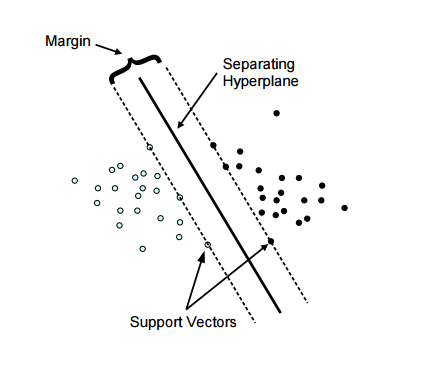
\includegraphics[width=0.6\textwidth]{figure/svm_wording.png}
 \end{minipage}
  \normalsize
 \begin{minipage}{0.5\textwidth}
 \centering
 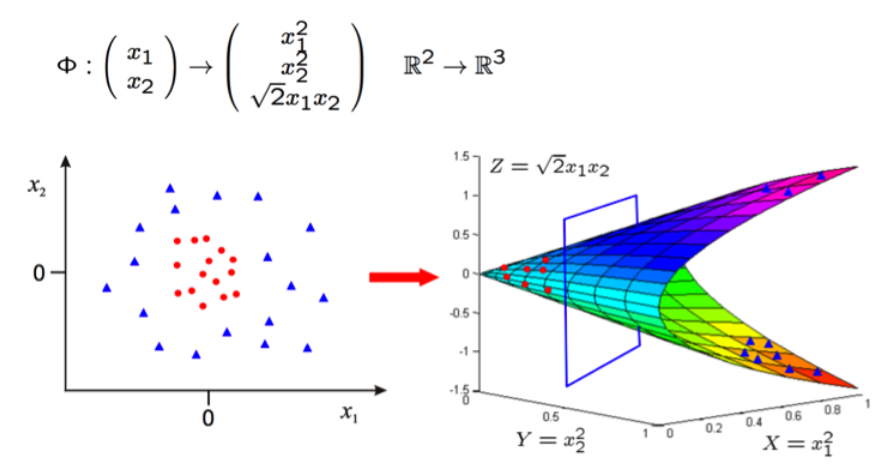
\includegraphics[width=0.6\textwidth]{figure/svm_kernel.PNG}
   
 \end{minipage}

\end{frame}

% ------------------------------------------------------------------------------

\LARGE
\begin{frame}{\textcolor{gray!80}{SVM} ~~ Functionality}
\normalsize
\vspace{-0.5cm}
\noindent \textcolor{gray!80}{\rule{\textwidth}{1pt}}

\vspace{0.3cm}

\footnotesize

\textbf{\textcolor{gray!80}{Empirical risk}}

N

\medskip

\textbf{\textcolor{gray!80}{Optimization}} ~~
XX

\medskip

\textbf{\textcolor{gray!80}{Hyperparameter}}

\begin{itemize}
  \item \textbf{C}: penalization for missclassified data points 
  \item \textbf{kernel parameters}: depending if and which kernel is used (e. g. degree of the polynomial kernel or width of RBF kernel)

\end{itemize}

\end{frame}

% ------------------------------------------------------------------------------

\LARGE
\begin{frame}{\textcolor{gray!80}{SVM} ~~ Pro's \& Con's}
\normalsize
\vspace{-0.5cm}
\noindent \textcolor{gray!80}{\rule{\textwidth}{1pt}}

\vspace{0.3cm}

\footnotesize


\begin{columns}[onlytextwidth]
  \begin{column}{0.5\textwidth}
    \textbf{\textcolor{gray!80}{Advantages}}
    \footnotesize
    \begin{itemize}
      \item[$\textbf{\textcolor{gray!80}{+}}$] can learn non-linear decision boundaries
      \item [$\textbf{\textcolor{gray!80}{+}}$] often sparse solution
      \item[$\textbf{\textcolor{gray!80}{+}}$] robust against overfitting; especially in high-dimensional space 
      \item[$\textbf{\textcolor{gray!80}{+}}$] computational costs are low ????? 
    \end{itemize}
  \end{column}

  \begin{column}{0.5\textwidth}
    \textbf{\textcolor{gray!80}{Disadvantages}}
    \footnotesize
    \begin{itemize}
      %\item[$\textbf{\textcolor{gray!80}{-}}$] very memory-intensive
      \item[$\textbf{\textcolor{gray!80}{-}}$] not easy tunable as it is highly important to choose the right kernel
      \item[$\textbf{\textcolor{gray!80}{-}}$] does not scale well to larger data sets
    \end{itemize}
  \end{column}
\end{columns}

\vfill

\small

\fbox{\parbox{\textwidth}{
\centering
\textbf{XX}}}

\end{frame}

% ------------------------------------------------------------------------------

\LARGE
\begin{frame}{\textcolor{gray!80}{SVM} ~~ Practical hints}
\normalsize
\vspace{-0.5cm}
\noindent \textcolor{gray!80}{\rule{\textwidth}{1pt}}

\vspace{0.3cm}

\footnotesize

  \textbf{\textcolor{gray!80}{Kernels}} \\
  \smallskip
 For projecting the input data into another onto a higher dimension, mainly these three types of kernels are used: 
 \begin{itemize}
 
 \item \textbf{Linear kernel}: the dot product of the given observations
 
 \item \textbf{Polynomial kernel}: curved lines in the input space
 
 \item \textbf{Radial basis function (RBF) kernel}: complex regions in the input space (e. g. spirals)
 
 \end{itemize}
 
 

\lz

  \textbf{\textcolor{gray!80}{Implementation}} \\
  \smallskip
  R: package for regularized linear model \texttt{XXX}\\
  Python: \texttt{XX} from package \texttt{XXX}, package for XXXX \texttt{statsmodels.api}

\end{frame}

% ------------------------------------------------------------------------------

% 
% ------------------------------------------------------------------------------
% NEURAL NETWORK
% ------------------------------------------------------------------------------

\LARGE
\begin{frame}{\textcolor{gray!80}{Neural Network} ~~ Functionality}
\normalsize
\vspace{-0.5cm}
\noindent \textcolor{gray!80}{\rule{\textwidth}{1pt}}

\vspace{0.3cm}

\footnotesize

\colorbox{gray!80}{\textcolor{white}{(UN)SUPERVISED}}
\colorbox{gray!80}{\textcolor{white}{(NON)PARAMETRIC}}
\colorbox{gray!80}{\textcolor{white}{BLACK-BOX}}
%\colorbox{gray!80}{\textcolor{white}{REGRESSION}}
%\colorbox{gray!80}{\textcolor{white}{FEATURE SELECTION}}

\medskip

\textbf{\textcolor{gray!80}{General idea}} ~~ A neural network (NN) is a model
architecture loosely inspired by the human brain. It consists of various
\textit{\textbf{neurons}} organized in \textit{\textbf{layers}}. These layers
are assembled through functional connections. 
\\ Data enter the network in
the \textit{\textbf{input layer}} and sequentially pass through one or various
\textit{\textbf{hidden layers}}, each of which performs some transformation of
its inputs. The \textit{\textbf{output layer}} receives the repeatedly
transformed inputs and computes a prediction based on these.

\medskip
 
\textbf{\textcolor{gray!80}{Hypothesis space}} ~~
$\Hspace = \left\{ \fx: \fx = \sum_{t = 1}^T c_t \I(\xv \in Q_t) 
\right\}$

\medskip

\begin{minipage}{0.6\textwidth}
  \begin{itemize}
    \item Pass observations along until each ends up in exactly 
    one leaf node
    \item In each step, find the optimal feature-threshold
    combination to \\ split by
  \item Assign response $c_t$ to leaf node $t$
\end{itemize}

\end{minipage}%
\begin{minipage}{0.4\textwidth}
  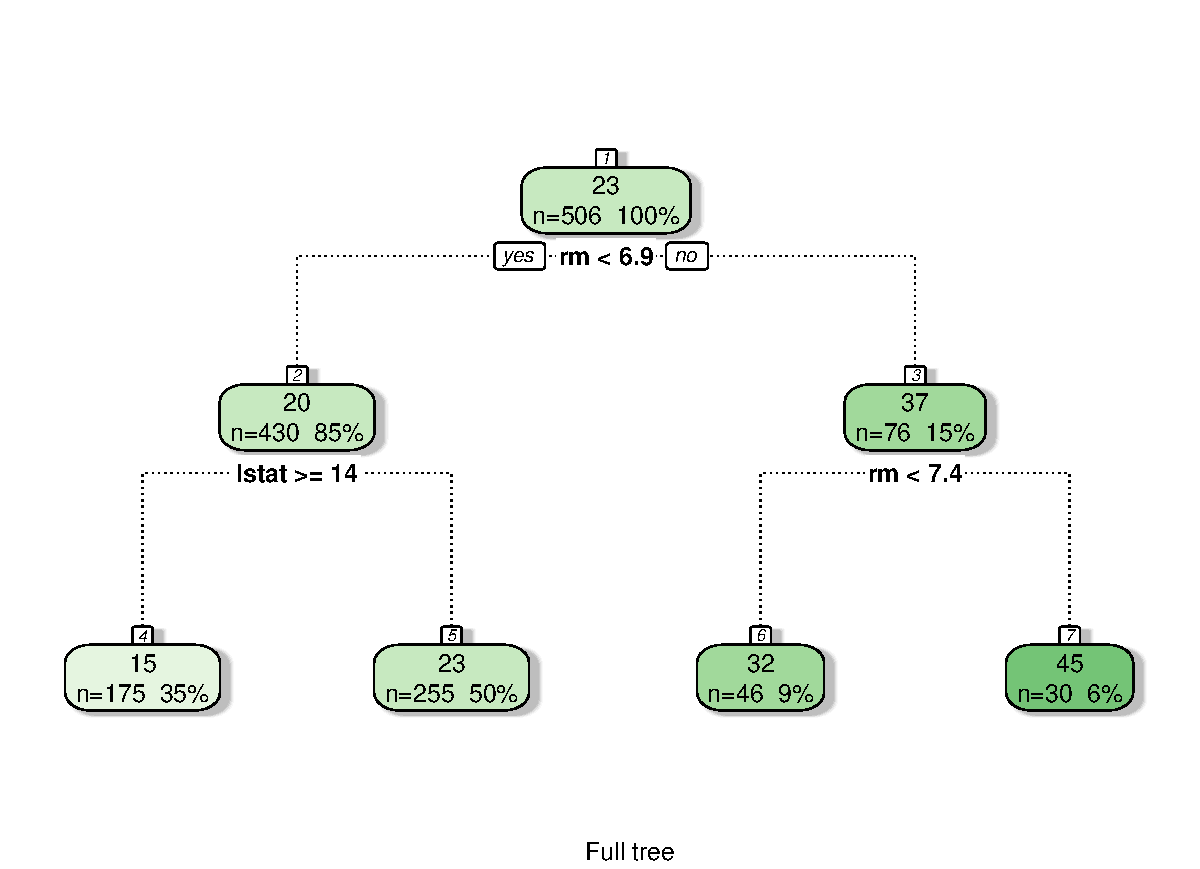
\includegraphics[width=\textwidth]{figure/cart.pdf}
\end{minipage}

% \begin{itemize}
% \item A neural network (NN) is a complex function or hypothesis space which loosly inspired by (very) loosely inspired by the organisation of
% neurons in biological brains.
% 
% \item A neural network consists of interconnected neurons which are organized in layers.
% 
% \item A \textbf{neuron} computes the weighted average of its input, and this sum is passed through a nonlinear function (\textbf{activation function}):
% \end{itemize}

\medskip
  \centering
  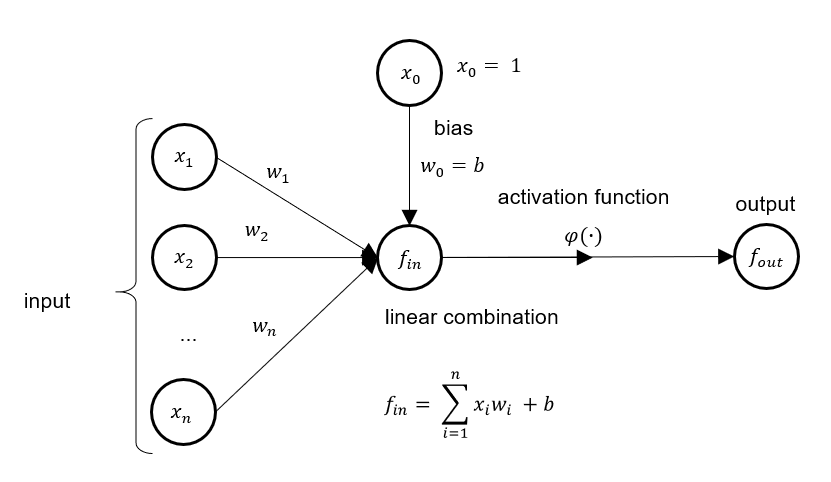
\includegraphics[width=0.5\textwidth]{figure/nn_neuron.PNG}

\end{frame}

% ------------------------------------------------------------------------------

\LARGE
\begin{frame}{\textcolor{gray!80}{Neural Network} ~~ Functionality}
\normalsize
\vspace{-0.5cm}
\noindent \textcolor{gray!80}{\rule{\textwidth}{1pt}}

\vspace{0.3cm}

\footnotesize

\begin{itemize}

\item NNs use "hidden layers" between inputs and outputs in order to model intermediary representations of the data: 

\end{itemize}



\medskip
  \centering
  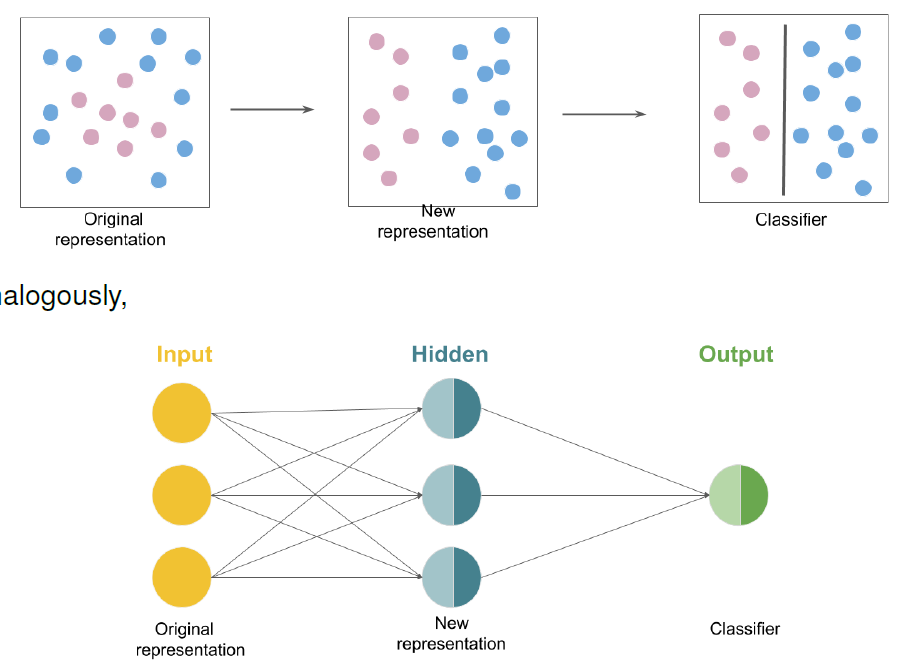
\includegraphics[width=0.3\textwidth]{figure/nn_representation_learning.png}


%\textbf{\textcolor{gray!80}{Hypothesis space}} ~~
%$\Hspace = \{ \theta_0 + \thx\ |\ (\theta_0, \thetab) \in \R^{p+1} \} $

\medskip
% \footnotesize
% \begin{minipage}{0.5\textwidth}
%\centering
  %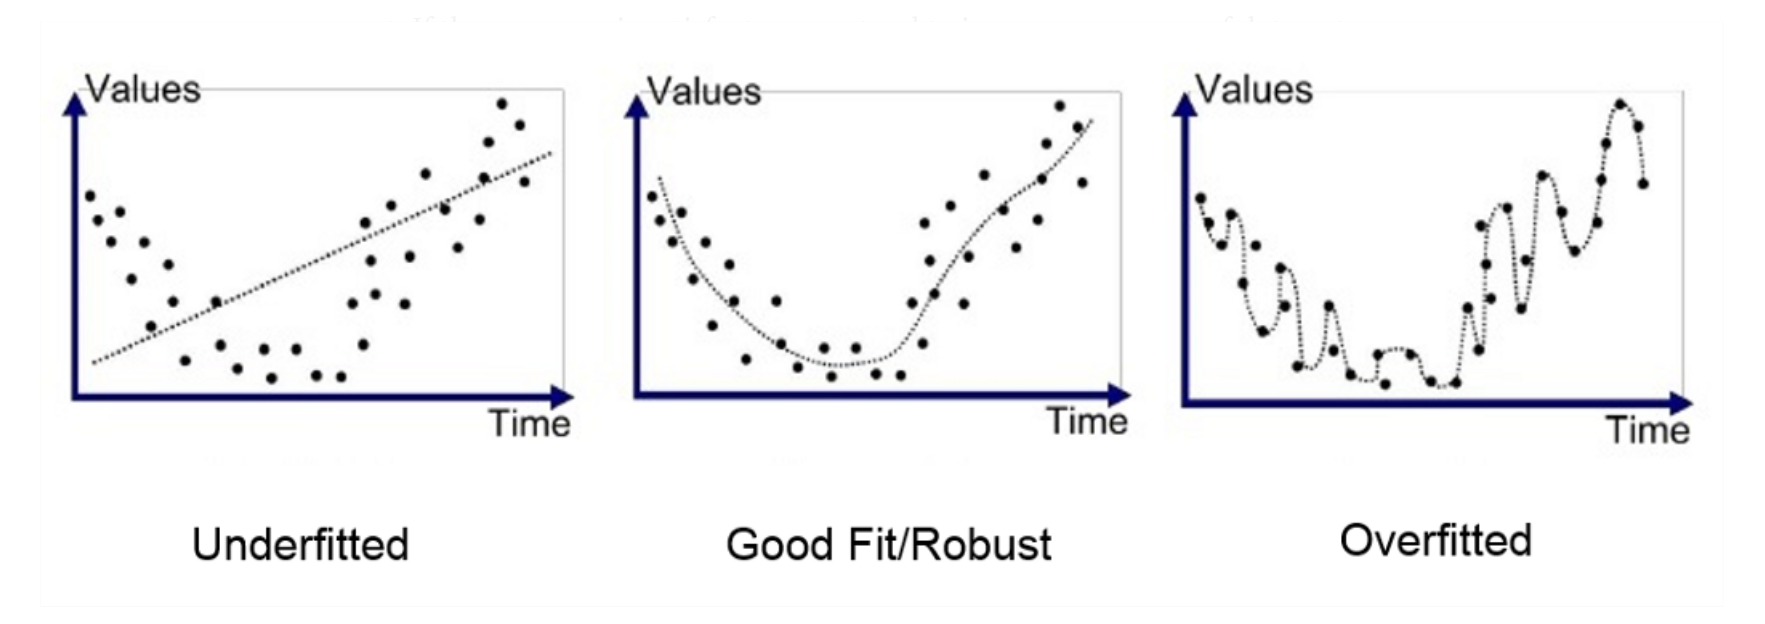
\includegraphics[width=0.7\textwidth]{figure/reg_lm_comparision.png}
% \end{minipage}
%  \normalsize
% \begin{minipage}{0.4\textwidth}
%   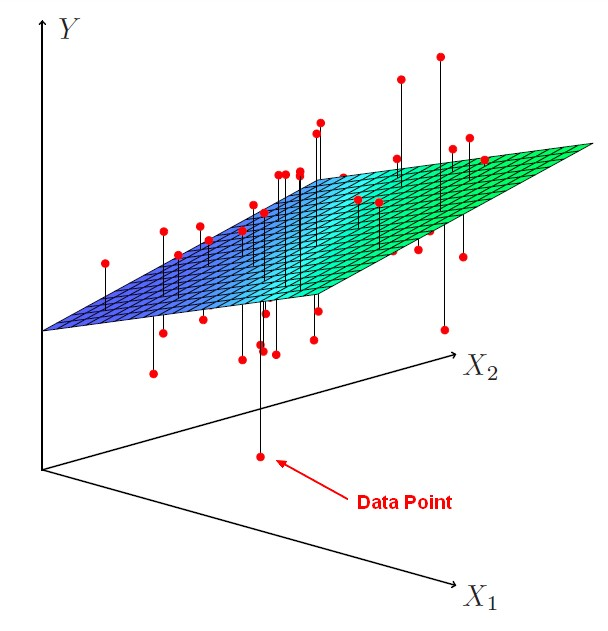
\includegraphics[width=0.7\textwidth]{figure/regression_hyperplane.jpg}
% \end{minipage}



\textbf{\textcolor{gray!80}{Empirical risk}} ~~ XX

%\begin{itemize}
% 
% \item XX
%   
%   
% \end{itemize}
% 
% 
 \medskip

\textbf{\textcolor{gray!80}{Optimization}} ~~ NNs are optimised by \textbf{backpropagation} which consists of two steps:
\begin{itemize}
  \item \textbf{Forward pass}: Predict result witch current weights and calculate empirical loss. 
  \item \textbf{Backward pass}: Calculate error contribution of each weight and update the weights by the negative gradient descent. 
\end{itemize}

\medskip

\textbf{\textcolor{gray!80}{Hyperparameters}} ~~ Number of hidden neurons, Dropout, initial weights, activation function, learning rate, number of epochs, batch size

\end{frame}

% ------------------------------------------------------------------------------

\LARGE
\begin{frame}{\textcolor{gray!80}{Neural Network} ~~ Pro's \& Con's}
\normalsize
\vspace{-0.5cm}
\noindent \textcolor{gray!80}{\rule{\textwidth}{1pt}}

\vspace{0.3cm}

\footnotesize


\begin{columns}[onlytextwidth]
  \begin{column}{0.5\textwidth}
    \textbf{\textcolor{gray!80}{Advantages}}
    \footnotesize
    \begin{itemize}
      \item[$\textbf{\textcolor{gray!80}{+}}$] can solve complex, non-linear regression or classification problems 
      \item[$\textbf{\textcolor{gray!80}{+}}$] also suitable for unstructed data (e. g. image, audio and text data)  
      \item[$\textbf{\textcolor{gray!80}{+}}$] very accuarate 
      \item[$\textbf{\textcolor{gray!80}{+}}$] can easily be updated %batch propagation
      \item[$\textbf{\textcolor{gray!80}{+}}$] reduces the need for feature engeneering
    \end{itemize}
  \end{column}

  \begin{column}{0.5\textwidth}
    \textbf{\textcolor{gray!80}{Disadvantages}}
    \footnotesize
    \begin{itemize}
      \item[$\textbf{\textcolor{gray!80}{-}}$] requires a huge amount of data
      \item[$\textbf{\textcolor{gray!80}{-}}$] black-model $\rightarrow$ hard to interpret or explain
      \item[$\textbf{\textcolor{gray!80}{-}}$] computationally expensive $\rightarrow$ slow to train and forecast
      \item[$\textbf{\textcolor{gray!80}{-}}$] tend to overfit
      \item[$\textbf{\textcolor{gray!80}{-}}$] requires much expertise for tuning
    \end{itemize}
  \end{column}
\end{columns}

\vfill

\small

\fbox{\parbox{\textwidth}{
\centering
\textbf{Computationally expensive models which can learn complex functions and are suitable for unstructred data like text or pictures.}}}

\end{frame}

% ------------------------------------------------------------------------------

\LARGE
\begin{frame}{\textcolor{gray!80}{Neural Network} ~~ Practical hints}
\normalsize
\vspace{-0.5cm}
\noindent \textcolor{gray!80}{\rule{\textwidth}{1pt}}

\vspace{0.3cm}

\footnotesize

\lz

  \textbf{\textcolor{gray!80}{RNNS}} \\
  \smallskip
 XXXX
 
 \textbf{\textcolor{gray!80}{CNNS}} \\
  \smallskip
 XXXX
 
 

\lz

  \textbf{\textcolor{gray!80}{Implementation}} \\
  \smallskip
  R: package for regularized linear model \texttt{XXX}\\
  Python: \texttt{XX} from package \texttt{XXX}, package for XXXX \texttt{statsmodels.api}

\end{frame}

% % ------------------------------------------------------------------------------
% 
% % 
% % % ------------------------------------------------------------------------------
% % % KNN 
% % % ------------------------------------------------------------------------------
% 
% \LARGE
% \begin{frame}{\textcolor{gray!80}{KNN} ~~ Functionality}
% \normalsize
% \vspace{-0.5cm}
% \noindent \textcolor{gray!80}{\rule{\textwidth}{1pt}}
% 
% \vspace{0.3cm}
% 
% \footnotesize
% 
% \colorbox{gray!80}{\textcolor{white}{SUPERVISED}}
% \colorbox{gray!80}{\textcolor{white}{PARAMETRIC}}
% \colorbox{gray!80}{\textcolor{white}{WHITE-BOX}}
% %\colorbox{gray!80}{\textcolor{white}{REGRESSION}}
% %\colorbox{gray!80}{\textcolor{white}{FEATURE SELECTION}}
% 
% \medskip
% 
% \textbf{\textcolor{gray!80}{General idea}} ~~
% \begin{itemize}
% 
% \item XX
% 
% \end{itemize}
% 
% \medskip
% 
% \textbf{\textcolor{gray!80}{Hypothesis space}} ~~
% %$\Hspace = \{ \theta_0 + \thx\ |\ (\theta_0, \thetab) \in \R^{p+1} \} $
% 
% \medskip
% % \footnotesize
% % \begin{minipage}{0.5\textwidth}
% \centering
%   %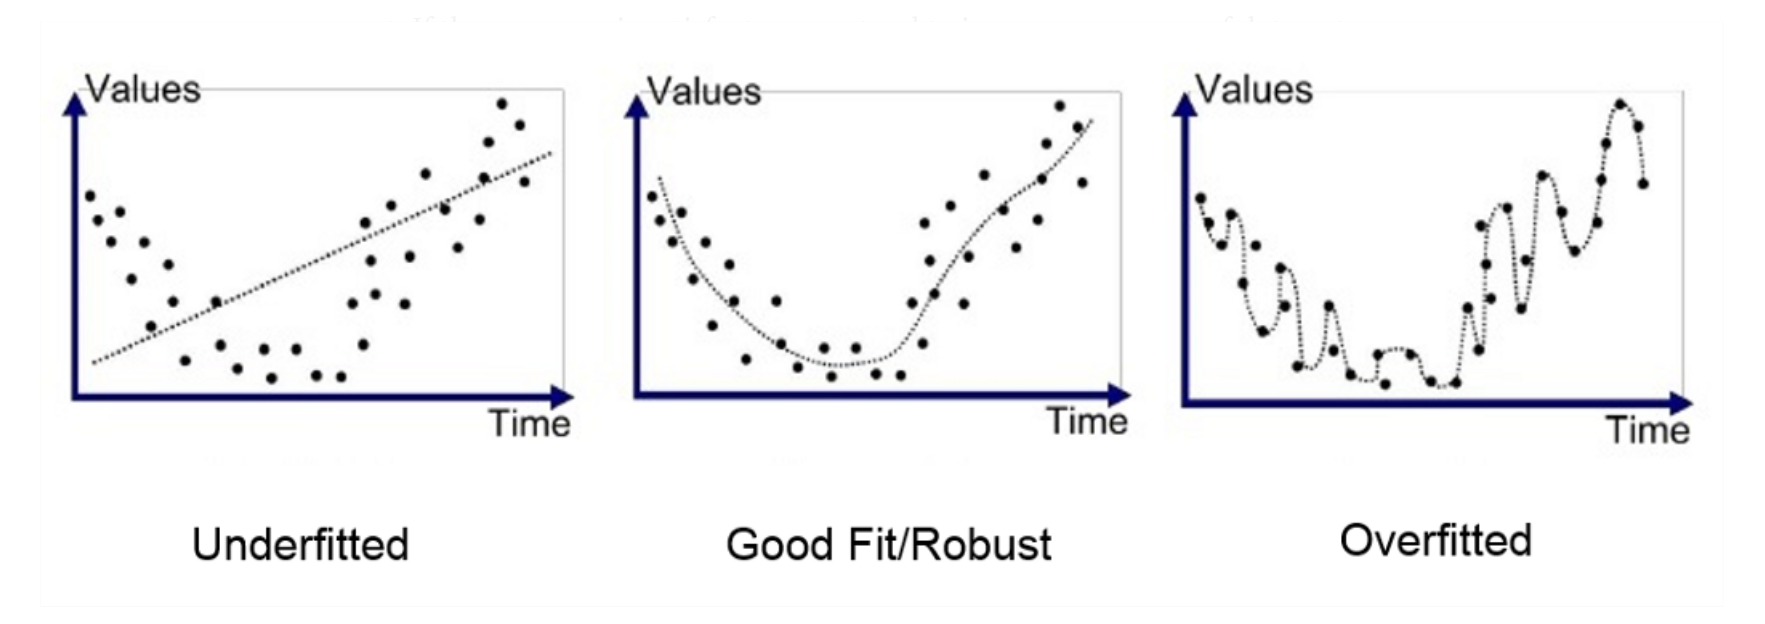
\includegraphics[width=0.7\textwidth]{figure/reg_lm_comparision.png}
% % \end{minipage}
% %  \normalsize
% % \begin{minipage}{0.4\textwidth}
% %   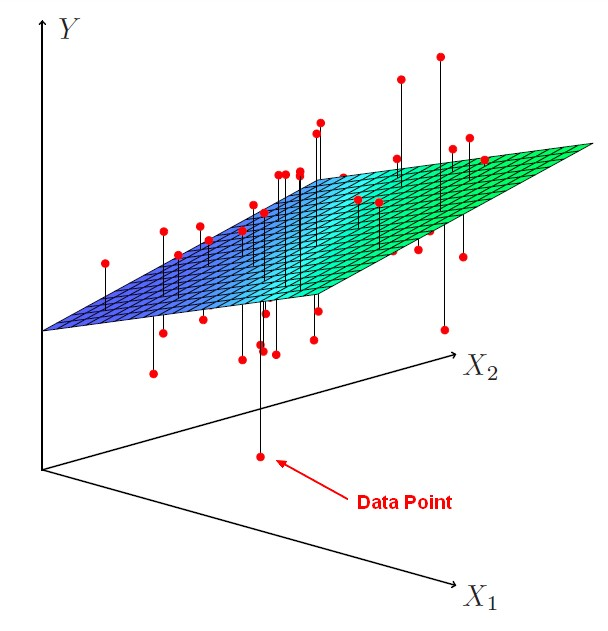
\includegraphics[width=0.7\textwidth]{figure/regression_hyperplane.jpg}
% % \end{minipage}
% 
% \end{frame}
% 
% % ------------------------------------------------------------------------------
% 
% \LARGE
% \begin{frame}{\textcolor{gray!80}{KNN} ~~ Functionality}
% \normalsize
% \vspace{-0.5cm}
% \noindent \textcolor{gray!80}{\rule{\textwidth}{1pt}}
% 
% \vspace{0.3cm}
% 
% \footnotesize
% 
% \textbf{\textcolor{gray!80}{Empirical risk}}
% 
% \begin{itemize}
% 
% \item XX
%   
%   
% \end{itemize}
% 
% 
% \medskip
% 
% \textbf{\textcolor{gray!80}{Optimization}} ~~
% XX
% 
% \medskip
% 
% \textbf{\textcolor{gray!80}{Hyperparameter}} XX
% 
% \end{frame}
% 
% % ------------------------------------------------------------------------------
% 
% 
% 
% 
% % \textbf{Advantages}
% % \begin{itemize}
% % \item simple adabtle to problem 
% % \item accuarate
% % \item easy to understand
% % \item few parameters to tune
% % \end{itemize}
% % 
% % 
% % \textbf{Disadvantages}
% % \begin{itemize}
% % \item memory intensive
% % \item computationally costly --> all training data might be involved in the decision making
% % \item slow performance
% % \item wrong distance measure can lead to inaccurate results 
% % \item k must be selected
% % \end{itemize}
% % \end{frame}
% 
% 
% 
% \LARGE
% \begin{frame}{\textcolor{gray!80}{KNN} ~~ Pro's \& Con's}
% \normalsize
% \vspace{-0.5cm}
% \noindent \textcolor{gray!80}{\rule{\textwidth}{1pt}}
% 
% \vspace{0.3cm}
% 
% \footnotesize
% 
% 
% \begin{columns}[onlytextwidth]
%   \begin{column}{0.5\textwidth}
%     \textbf{\textcolor{gray!80}{Advantages}}
%     \footnotesize
%     \begin{itemize}
%       \item[$\textbf{\textcolor{gray!80}{+}}$] XX
%     \end{itemize}
%   \end{column}
% 
%   \begin{column}{0.5\textwidth}
%     \textbf{\textcolor{gray!80}{Disadvantages}}
%     \footnotesize
%     \begin{itemize}
%       \item[$\textbf{\textcolor{gray!80}{-}}$] XX
%     \end{itemize}
%   \end{column}
% \end{columns}
% 
% \vfill
% 
% \small
% 
% \fbox{\parbox{\textwidth}{
% \centering
% \textbf{XX}}}
% 
% \end{frame}
% 
% % ------------------------------------------------------------------------------
% 
% \LARGE
% \begin{frame}{\textcolor{gray!80}{KNN} ~~ Practical hints}
% \normalsize
% \vspace{-0.5cm}
% \noindent \textcolor{gray!80}{\rule{\textwidth}{1pt}}
% 
% \vspace{0.3cm}
% 
% \footnotesize
% 
%   \textbf{\textcolor{gray!80}{Choice of regularization parameter  $\lambda$}} \\
%   \smallskip
%  XXXX
%  
%  
% 
% \lz
% 
%   \textbf{\textcolor{gray!80}{Implementation}} \\
%   \smallskip
%   R: package for regularized linear model \texttt{XXX}\\
%   Python: \texttt{XX} from package \texttt{XXX}, package for XXXX \texttt{statsmodels.api}
% 
% \end{frame}
% 
% % ------------------------------------------------------------------------------











\endlecture

\end{document}








